\themaN
\graphicspath{{../Ch27_Pourcentages_echelles_vitesse/Images/}}

\chapter{Pourcentages\\et échelles}
\label{C17}

%%%%%%%%%%%%%%%%%%%%%%%%%%%%%%%%%%%%%%%%%%
\begin{prerequis}[Connaissances et compétences abordées]
   \begin{itemize}
     \item Appliquer un pourcentage.
   \end{itemize}
\end{prerequis}

\vfill

\begin{debat}[Débat : le symbole du pourcentage] 
   Dans les textes du Moyen Âge, on peut voir des notations comme \og per cento \fg{} ou \og per c. \fg{} ou \og p. cento \fg. La première trace d'un symbole voisin de celui utilisé actuellement se trouverait dans un manuscrit italien anonyme, écrit vers 1425, sous la forme : $P.c$\degre. \\
   Le \og $P$ \fg{} s'est ensuite perdu, et on trouve, vers 1650, la notation : $\dfrac{o}{o}$, puis la barre est devenue oblique. Les deux \og o \fg{} sont ensuite assimilés aux deux zéros de 100. \\
   \begin{center}
      \textcolor{B1}{\fontsize{70}{80}\selectfont \%}
   \end{center}
   \bigskip
   \begin{cadre}[B2][F4]
      \begin{center}
         Vidéos : \href{https://www.youtube.com/watch?v=ibWzdm_05zs}{\bf Consommation d'huile de palme} et \href{https://www.youtube.com/watch?v=gLbsxj8mv-U}{\bf Facture d'électricité}, issues de journaux télévisés.
      \end{center}
   \end{cadre}
\end{debat}

\vfill

\textcolor{PartieGeometrie}{\sffamily\bfseries Cahier de compétences} : chapitre 5, exercices 24 à 36 ; 41 ; 42.


%%%%%%%%%%%%%%%%%%%%%%%%%%%%%%
%%%%%%%%%%%%%%%%%%%%%%%%%%%%%%
\activites

\begin{activite}[Carte, échelle]
   {\bf Objectifs :} calculer des distances ; résoudre un problème d'échelle.
   \begin{QCM}
      \begin{center}
         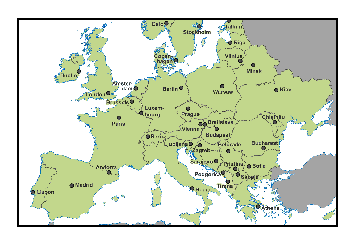
\includegraphics[width=16cm]{europe}
      \end{center}
      \partie[Quelques distances]
         Sachant que la distance à vol d'oiseau de Lisbonne à Amsterdam est de \ukm{1800}, répondre aux questions suivantes :
         \begin{enumerate}
            \item Quelle est la distance de Lisbonne à Paris ? \pf \smallskip
            \item Quelle est la distance de Paris à Oslo ? \pf \smallskip
            \item Quelle est la distance de Londres à Dublin ? \pf \\
         \end{enumerate}
    
      \partie[Construction de l'échelle]
      \vspace*{-5mm}
         \begin{enumerate}
            \item À combien de kilomètres dans la réalité correspond 1 centimètre sur la carte ? \pf \smallskip
            \item Par combien de centimètres sur la carte sont représentés 500 km dans la réalité ? \pf \smallskip
            \item Ajouter une échelle sur la carte.
         \end{enumerate}

      \partie[Tableau récapitulatif]
         \begin{center}
            {\small
            \hautab{1.2}
            \begin{Ctableau}{0.95\linewidth}{7}{c}
               \hline
               Trajet & Lisb.-Ams. & Lisb.-Paris & Paris-Oslo & Lond.-Dub. & & \\
                \hline
               Distance réelle en km & & & & & 200 & \\
               \hline
               Distance sur la carte en cm & & & & & & 1 \\
               \hline
           \end{Ctableau}} \medskip
         \end{center}
   \end{QCM}
\end{activite}


%%%%%%%%%%%%%%%%%%%%%%%%%%%%%%%%%%%%%
%%%%%%%%%%%%%%%%%%%%%%%%%%%%%%%%%%%%%
\cours 

%%%%%%%%%%%%%%%%% 1 %%%%%%%%%%%%%%%
\section{Pourcentages}

\begin{definition}
   Le {\bf pourcentage} d'une quantité est le nombre qui aurait été proportionnellement obtenu si la quantité avait été de 100.
\end{definition}

\begin{propriete}
   Pour calculer le pourcentage $p\,\%$ d'une quantité, on multiplie la quantité par $\dfrac{p}{100}$.
\end{propriete}

\begin{exemple}
   Un jeu à 39 \euro{} est en promotion à $-$20\,\%. 
   \begin{itemize}
      \item Quel est le montant de la remise ?
      \item Quel est le prix du jeu après remise ?
   \end{itemize}
   \correction
   \ \\ [-8mm]
   \begin{itemize}
      \item Calcul de la remise : $\dfrac{20}{100}\times\ueuro{39}=\ueuro{7}$. \medskip
      \item Calcul du nouveau prix : $\ueuro{39}-\ueuro{7,8} =\ueuro{31,2}$.
   \end{itemize}
\end{exemple}

\bigskip

Pourcentages simples : \\
$\bullet$ 10\,\% d'une quantité correspond à un dixième de cette quantité. \\
$\bullet$ 25\,\% d'une quantité correspond à un quart de cette quantité. \\
$\bullet$ 50\,\% d'une quantité correspond à la moitié de cette quantité. \\
$\bullet$ 75\,\% d'une quantité correspond aux trois quarts de cette quantité. \\
$\bullet$ 100\,\% d'une quantité correspond à la totalité de la quantité. \\

\begin{center}
   \begin{pspicture}(-1.5,-1.5)(2,1.5)
      \pscircle(0,0){1.5}
      \pswedge[fillstyle=solid,fillcolor=B1](0,0){1.5}{0}{90}
      \rput(0.75,0.75){\white 25\,\%}
   \end{pspicture}
   \begin{pspicture}(-1.5,-1.5)(2,1.5)
      \pscircle(0,0){1.5}
      \pswedge[fillstyle=solid,fillcolor=B1!80](0,0){1.5}{0}{180}
      \rput(0,0.75){\white 50\,\%}
   \end{pspicture}
   \begin{pspicture}(-1.5,-1.5)(2,1.5)
      \pscircle(0,0){1.5}
      \pswedge[fillstyle=solid,fillcolor=B1!60](0,0){1.5}{0}{-90}
      \rput(-0.75,0.75){\white 75\,\%}
   \end{pspicture}
   \begin{pspicture}(-1.5,-1.5)(2,1.5)
      \pscircle[fillstyle=solid,fillcolor=B1!40](0,0){1.5}
      \rput(0,0){\white 100\,\%}
   \end{pspicture}
\end{center}


%%%%%%%%%%%%%%%%% 2 %%%%%%%%%%%%%%%
\section{Echelles}

\begin{definition}
   L'\textbf{échelle} d'une carte est le rapport entre une longueur sur la carte et la longueur réelle sur le terrain.
\end{definition}

\smallskip

\begin{exemple}
   Représenter un champ carré \um{20} de côté à l'échelle 1/1000\up{e}.
   \correction
   \ucm{1000} dans la réalité, c'est à dire \um{10} sont représentés par \ucm{1} sur la feuille, il faut donc tracer un carré de \ucm{2} de côté.
   \begin{center}
      \begin{pspicture}(0,0)(2,2)
         \psframe(0,0)(2,2)
      \end{pspicture}
   \end{center}
\end{exemple}



%%%%%%%%%%%%%%%%%%%%%%%%%%%%%%%%%%%%%%
\exercicesbase

\begin{colonne*exercice}

\serie{Pourcentages} %%%%%

\begin{exercice} %1
   Recopier les phrases suivantes comme dans l'exemple : \\ [1mm]
   $\dfrac{10}{100} =\dfrac{1}{10}$ : 10\,\% représente un dixième d'une quantité. \bigskip
   \begin{enumerate}
      \item $\dfrac{20}{100} =\pfh$ : 20\,\% représente \pfb d'une quantité. \bigskip
      \item $\dfrac{25}{100} =\pfh$ : 25\,\% représente \pfb d'une quantité. \bigskip
      \item $\dfrac{50}{100} =\pfh$ : 50\,\% représente \pfb d'une quantité. \bigskip
      \item $\dfrac{75}{100} =\pfh$ : 75\,\% représente \pfb d'une quantité. \bigskip
      \item $\dfrac{100}{100} =\pfh$ : 100\,\% représente \pfb d'une quantité. \bigskip
      \item $\dfrac{200}{100} =\pfh$ : 200\,\% représente \pfb d'une quantité. \\
   \end{enumerate}
\end{exercice}


\begin{exercice} %2
   Calculer les pourcentages suivants mentalement.
   \begin{colenumerate}{2}
      \item 1\,\% de 50.
      \item 50\,\% de 60.
      \item 100\,\% de 7.
      \item 0,1\,\% de 650.
      \item 10\,\% de 250.
      \item 25\,\% de 400.
      \item 0\,\% de 15,4.
      \item 200\,\% de 15.
      \item 75\,\% de 44.
      \item \, 150\,\% de 8. \\
   \end{colenumerate}
\end{exercice}


\begin{exercice} %3
   Calculer en détaillant les étapes.
   \begin{colenumerate}{2}
      \item 29\,\% de 93.
      \item 35\,\% de 400.
      \item 20\,\% de 720.
      \item 87\,\% de 625.
      \item 7\,\% de 2\,000.
      \item 12\,\% de 500.
      \item 3\,\% de 5\,000.
      \item 151\,\% de 80. \\
   \end{colenumerate}
\end{exercice}


\begin{exercice} %4
   À la rentrée, une calculatrice graphique coûtait 59~\euro. À la Toussaint, son prix avait augmenté de 20\,\%. Pendant les fêtes de noël, il a baissé de 20\,\%.
   \begin{enumerate}
      \item Sans faire de calcul, pensez-vous que le prix après les fêtes est revenu a son prix initial de 59\,\euro ?
      \item Calculer l'augmentation à la Toussaint, en déduire son prix après augmentation.
      \item Calculer la réduction due aux fêtes de noël, en déduire son nouveau prix.
      \item Vérifier la réponse donnée en question 1).
\end{enumerate}
\end{exercice}


%\begin{exercice} %5
%   Au collège Simone Veil, il y a 650 élèves. 38\,\% d'entre eux sont demi-pensionnaires.
%   \begin{enumerate}
%      \item Quel est le pourcentage d'élèves externes ?
%      \item Calculer de deux façons différentes le nombre d'élèves externes. \\
%   \end{enumerate}
%\end{exercice}


\begin{exercice} %6
   Au collège Hélène Ordik, on a relevé les mentions au DNB parmi les 123 élèves ayant été reçus en 2019.
   \begin{center}
      {\hautab{1.3}
      \small
      \begin{ltableau}{0.9\linewidth}{3}
         \hline
         Mention AB & Mention B & Mention TB \\
         \hline
          33,66\,\% & 24,04\,\% & 11,54\,\% \\
         \hline
      \end{ltableau}}
      \vspace*{-3mm}
   \end{center}
   \begin{enumerate}
      \item Calculer le nombre d'élèves ayant eu une mention AB, B et TB.
      \item Calculer le pourcentage d'élèves n'ayant pas eu de mention.
      \item Calculer de deux façons différentes le nombre d'élèves n'ayant pas eu de mention. \\
   \end{enumerate}
\end{exercice}


\serie{Echelles} %%%%%
   
\begin{exercice} %7
   \begin{enumerate}
      \item Sur un plan d'un appartement à l’échelle 1/100\up{e}, la salle à manger est représentée par un rectangle de 8 cm de long sur 6 cm de large. Quelles sont les dimensions réelles de cette pièce ?
      \item Sur le plan d'un chalet, les portes sont représentées par un segment de 1,6 cm de long. En réalité, elles sont larges de 0,80 m. Quelle est l'échelle de ce plan ? \\
   \end{enumerate}
\end{exercice}


\begin{exercice} %8
On souhaite reproduire sur le cahier la cocotte et le bateau en multipliant toutes les longueurs par 4 tiers pour la cocotte et par un demi pour le bateau. 
   \begin{enumerate}
      \item Pour la cocotte, combien devra mesurer un segment de longueur 3 unités sur le cahier ? Même question pour un segment de mesure 1,5 unité ?
      \item Pour le bateau, combien devra mesurer un segment de longueur 4 unités sur le cahier ? Même question pour un segment de mesure 0,5 unité ?
   \end{enumerate}
   \begin{center}
      \psset{unit=0.5}
      \begin{pspicture}(17,10)
         \psgrid[subgriddiv=1,linestyle=solid,gridlabels=0,gridcolor=gray](0,0)(17,11)
         \psset{linewidth=0.45mm}
         \pspolygon(1,1)(4,1)(5.5,2.5)(7,1)(7,4)(5.5,5.5)(7,7)(4,7)(4,4)
         \pspolygon(8,3)(10,1)(14,1)(16,3)
         \psline(12,3)(12,10)(14,10)(14,9)(12,9)
         \psline(12,4)(8,4)(12,8)   
      \end{pspicture}
   \end{center} 
\end{exercice}

\end{colonne*exercice}


%%%%%%%%%%%%%%%%%%%%%%%%%%%%%%%%
%%%%%%%%%%%%%%%%%%%%%%%%%%%%%%%%
\Recreation

\enigme[Tableaux en fils tendus]
   Reproduire les deux tableaux 1 et 2 suivants de sorte que chaque figure ait une dimension de \ucm{10} par \ucm{10}.
   \begin{center}
      {\psset{unit=0.3}      
      \begin{pspicture}(-10,-10)(11,13)
         %\psgrid[gridlabels=0,subgriddiv=0,gridcolor=lightgray](-10,-10)(10,10)
         \rput(0,12){Tableau 1}
         \multido{\n=0+1,\i=10+-1}{11}{\psline(-10,\n)(-\i,10) %NOe
                                                         \psline(10,\n)(\i,10) %NEe
                                                         \psline(-10,-\n)(-\i,-10) %SOe
                                                         \psline(10,-\n)(\i,-10) %SEe
                                                         \psline(-\i,0)(0,\n) %NOi
                                                         \psline(\i,0)(0,\n) %NEi
                                                         \psline(\i,0)(0,-\n) %SEi
                                                         \psline(-\i,0)(0,-\n) %SEi
                                                        }
      \end{pspicture}}
      {\psset{unit=0.85,linecolor=PartieStatistique}
      \begin{pspicture}(-11,0)(0,10)
         %\psgrid[gridlabels=0,subgriddiv=0,gridcolor=lightgray](-10,-10)(10,10)
         \rput(-5,5){\textcolor{PartieStatistique}{détail du tableau 1}}
         \multido{\n=0+1,\i=10+-1}{11}{\psline(-10,\n)(-\i,10) %NOe
                                                         \psline(-\i,0)(0,\n) %NOi
                                                        }
      \end{pspicture}} \\ [10mm]
       {\psset{unit=0.55}
       \begin{pspicture}(-10,-9)(10,10)
       \psframe(-10,-10)(10,10)
          \rput(0,-8){Tableau 2}
          \multido{\n=0+1,\i=10+-1}{11}{\psline(-\i,-\i)(-\n,\n) %O
                                                      \psline(\i,\i)(\n,-\n) %E
                                                      \psline(-\i,\i)(\n,\n) %N
                                                      \psline(-\i,-\i)(\n,-\n) %S
                                                     }
      \end{pspicture}}
   \end{center}

